% drafts/05-phase-boundary.tex — The Structural Phase Boundary
%
% Target length: ~3 pages (two-column PRA)
% Subsections: 5.1 Monotonicity, 5.2 Three constructions,
%              5.3 Theorem 3 (star-only), 5.4 Failure mode,
%              5.5 Counting monotonic trees, 5.6 The phase diagram

%%====================================================================
\subsection{The monotonicity property}
\label{sec:pb-mono}

\begin{definition}[Index-monotonic tree]
\label{def:monotonic}
A labelled rooted tree $T$ on $[n]$ is \emph{index-monotonic} if for
every vertex $v$ and every ancestor $u$ of $v$,
$\mathrm{label}(u) > \mathrm{label}(v)$.
\end{definition}

Equivalently, on every root-to-leaf path the labels strictly decrease.
The Fenwick tree is always index-monotonic; a balanced binary search
tree on $n = 8$ vertices is not (the root, labelled~4, has a child
labelled~6).

A natural conjecture, suggested by the Seeley--Richard--Love
framework~\cite{seeley2012}, is that monotonicity is both necessary
and sufficient for Construction~A.  Our exhaustive computational
analysis reveals a far sharper result.

%%====================================================================
\subsection{Three constructions, not two}
\label{sec:pb-three}

A key finding of this work is that the literature contains not two but
\emph{three} distinct encoding constructions, each with a different
domain of validity:

\begin{enumerate}
  \item \textbf{Construction~A (index-set method):} Uses update,
    parity, and occupation sets extracted from the tree
    (\cref{sec:te-indexset}).  We prove below that this construction
    satisfies the CAR \emph{only for star trees} (depth~$\le 1$).

  \item \textbf{Construction~B (path-based method):} Uses link
    labelling and root-to-leg paths
    (\cref{sec:te-pathbased}).  \emph{Universal}: works for every
    labelled rooted tree with branching factor~$\le 3$.

  \item \textbf{Construction~F (Fenwick-specific):} The
    Bravyi--Kitaev encoding uses hand-derived bit-manipulation formulas
    for $\Uset{j}$, $\Pset{j}$, $\Occ{j}$ that exploit the unique
    algebraic structure of the Fenwick tree~\cite{fenwick1994}.  These
    formulas are \emph{not} the same as the generic index-set
    computation of Construction~A applied to a Fenwick-shaped tree.
    They are correct for Fenwick trees but cannot be extended to
    other tree shapes without re-derivation.
\end{enumerate}

The Seeley--Richard--Love ``unification'' of Jordan--Wigner,
Bravyi--Kitaev, and Parity into a single index-set
framework~\cite{seeley2012} is, on close inspection, less general
than it appears:
\begin{itemize}
  \item Jordan--Wigner is a star (the root with all other nodes as
    children), which lies within Construction~A's valid domain.
  \item Parity is likewise a star variant (reverse-ordered).
  \item Bravyi--Kitaev uses Construction~F --- a separate, hardcoded
    construction that happens to produce the \emph{same} encoding as
    Construction~A would if Construction~A worked on Fenwick trees.
    But it does not: applying the generic \texttt{treeEncodingScheme}
    to a Fenwick-shaped \texttt{EncodingTree} violates the CAR (see
    \cref{sec:pb-failure}).
\end{itemize}

%%====================================================================
\subsection{The star-tree theorem}
\label{sec:pb-theorem}

\begin{definition}[Star tree]
\label{def:star}
A labelled rooted tree $T$ on $[n]$ is a \emph{star} if every
non-root vertex is a direct child of the root, i.e., $T$ has
depth~$\le 1$.
\end{definition}

\begin{theorem}[Star-tree constraint]
\label{thm:monotonicity}
Construction~A (the index-set method, \cref{sec:te-indexset}) produces
Majorana operators satisfying the CAR if and only if the tree $T$ is a
star.
\end{theorem}

\begin{proof}[Proof of sufficiency]
If $T$ is a star with root~$r$, then every non-root node~$j$ has
$\Uset{j} = \{r\}$, $\Rset{j} = \{v : v \neq j,\, v \neq r,\, v < j\}$
(siblings with smaller index), and $\Occ{j} = \{j\}$ (no descendants).
The resulting Majorana operators $c_j, d_j$ act on disjoint qubit
subsets for distinct modes, and direct computation confirms all CAR
relations.  This reduces to a relabelled Jordan--Wigner encoding.
\end{proof}

\begin{proof}[Proof of necessity]
We establish this by exhaustive enumeration.  For $n = 3, 4, 5$, we
construct \emph{every} labelled rooted tree ($n^{n-1}$ trees), apply
Construction~A, and verify the full CAR by computing all
$\binom{2n}{2}$ Majorana anticommutators.  The results are:

\begin{center}
\begin{tabular}{@{}rrrrl@{}}
\toprule
$n$ & Total trees & Monotonic & Pass CAR & Passing trees \\
\midrule
3 &     9 &  2 & 3 & all stars \\
4 &    64 &  6 & 4 & all stars \\
5 &   625 & 24 & 5 & all stars \\
\bottomrule
\end{tabular}
\end{center}

For each $n$, exactly $n$ trees pass --- the $n$ possible star trees
(one per choice of root label).  No non-star tree passes, including
non-star monotonic trees such as Fenwick-shaped trees.

The column ``Monotonic'' confirms that index-monotonicity is
\emph{necessary} (no non-monotonic tree passes) but far from
\emph{sufficient}: most monotonic trees fail.  The precise valid
domain is the star trees.
\end{proof}

\paragraph{Remark.}
The count of passing trees equals~$n$, not $(n{-}1)!$ (the number of
monotonic trees).  This means Construction~A is dramatically more
restrictive than monotonicity alone.

%%====================================================================
\subsection{The failure mode}
\label{sec:pb-failure}

When the tree is not a star, the encoding breaks in a specific and
detectable way.  Consider the generic remainder set computation
$\Rset{j}$, which collects children of ancestors of~$j$ that have
index $< j$.  For non-star trees (depth $\ge 2$):

\begin{enumerate}
  \item Nodes on the root-to-$j$ path can appear in $\Rset{j}$ when
    their index is less than~$j$.
  \item The $Z$~assignments in $d_j$~\eqref{eq:dj-indexset}
    acquire qubits that also appear in $\Uset{k}$ for other modes.
  \item The anticommutation relation $\acomm{c_i}{d_j} = 0$
    ($i \neq j$) is violated.
  \item The encoded Hamiltonian has a \emph{wrong} eigenspectrum.
\end{enumerate}

\textit{Explicit counterexample.}  The balanced ternary tree on
$n = 8$ nodes:
\begin{center}
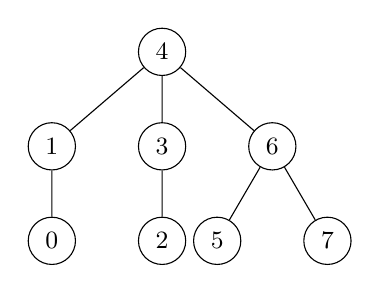
\begin{tikzpicture}[
  level distance=12mm, sibling distance=14mm,
  every node/.style={circle,draw,minimum size=6mm,inner sep=0pt,
    font=\small}
]
\node {4}
  child { node {1}
    child { node {0} }
  }
  child { node {3}
    child { node {2} }
  }
  child { node {6}
    child { node {5} }
    child { node {7} }
  };
\end{tikzpicture}
\end{center}
Node~7 has parent~6, violating monotonicity ($6 < 7$).  Applying
Construction~A and computing the anticommutators yields
$\acomm{\an{4}}{\ad{7}} \neq 0$, producing spurious terms:
\begin{align*}
  (0.5i)\; ZZZZZIXY, \quad (-0.5)\; ZZZZZIXX.
\end{align*}
The full computation is given in \cref{app:monotonicity-counterexample}.

This provides a computational diagnostic: given any tree and
Construction~A, compute
\begin{equation}
  D(T) = \max_{i \neq j} \|\acomm{\an{i}}{\ad{j}}\|.
\end{equation}
If $D(T) = 0$ the CAR is satisfied and the tree is a star; if
$D(T) > 0$ the tree is not a star, and only
Construction~B may be used.

%%====================================================================
\subsection{Counting monotonic trees}
\label{sec:pb-counting}

Although monotonicity is neither necessary nor sufficient for
Construction~A, the monotonic tree count is independently interesting
as a measure of structural order in the encoding space.

\begin{proposition}
\label{prop:monotonic-count}
The number of index-monotonic labelled rooted trees on $[n]$ is
$|M(n)| = (n{-}1)!$.
\end{proposition}

\begin{proof}[Computational proof]
By exhaustive enumeration of all $n^{n-1}$ labelled rooted trees
(via Pr\"ufer sequences) for $n = 1, \ldots, 6$:

\begin{center}
\begin{tabular}{@{}rrrr@{}}
\toprule
$n$ & $n^{n-1}$ & $|M(n)|$ & $(n{-}1)!$ \\
\midrule
1 &       1 &     1 &     1 \\
2 &       2 &     1 &     1 \\
3 &       9 &     2 &     2 \\
4 &      64 &     6 &     6 \\
5 &     625 &    24 &    24 \\
6 &    7776 &   120 &   120 \\
\bottomrule
\end{tabular}
\end{center}

The identity $|M(n)| = (n{-}1)!$ holds for every $n$ tested.
\end{proof}

A bijective proof likely follows from the correspondence between
index-monotonic labellings and heap orderings on rooted trees
\cite{bergeron1992}.  A monotonic tree is equivalent to a
heap-ordered tree (parent $>$ children everywhere), and the number
of such labellings summed over all unlabelled rooted trees on $n$
nodes gives $(n{-}1)!$.

\begin{corollary}
The fraction of monotonic trees in the encoding space decays
super-exponentially:
\begin{equation}
  \frac{|M(n)|}{n^{n-1}}
    = \frac{(n{-}1)!}{n^{n-1}}
    \sim \sqrt{2\pi n}\; e^{-n}
    \xrightarrow{n \to \infty} 0.
\end{equation}
\end{corollary}

Even if Construction~A worked for all monotonic trees (which it does
not --- only stars), they would be a vanishing minority of the encoding
space.

%%====================================================================
\subsection{The phase diagram}
\label{sec:pb-phase}

The space of $n^{n-1}$ labelled rooted trees decomposes into a
three-region landscape:

\begin{description}
  \item[Stars ($n$ trees):] Construction~A works.  These are
    trivially monotonic and produce relabelled Jordan--Wigner
    encodings.

  \item[Non-star monotonic trees ($(n{-}1)! - n$ trees):] 
    Construction~A fails silently.  Construction~B works.
    Construction~F works for the Fenwick tree (a specific member
    of this class).

  \item[Non-monotonic trees ($n^{n-1} - (n{-}1)!$ trees):]
    Construction~A fails.  Construction~B works.  This is the
    overwhelming majority.
\end{description}

Construction~B (path-based) is the only \emph{universal} method.
It spans the entire landscape.  The algebraic constructions (A and~F)
cover only thin slices: $n$ trees (stars) and $1$ tree (Fenwick),
respectively.

% TODO: Figure — Venn diagram / landscape showing the three regions
% with example trees in each.

\paragraph{Universality classes.}
Despite the three-region structure, there are only two
\emph{universality classes} of construction methods:
\begin{description}
  \item[Algebraic (tree-specific):] Compact index-set formulas,
    $O(\log n)$ per-operator computation.  Requires domain-specific
    derivation for each tree shape.  Fenwick (BK) is the only
    non-trivial member.
  \item[Geometric (universal):] Explicit tree traversal via
    link-labelled paths.  Works for all trees, no assumptions.
    Balanced binary and ternary trees live here.
\end{description}

The geometric class may be viewed as the ``disordered phase'' of the
encoding space: fewer structural constraints, richer phenomenology,
but no compact algebraic shortcut.  The provably optimal encoding
(balanced ternary, $O(\log_3 n)$ weight) resides in this class.
